\subsubsection{rendering.tick.dynamics.properties}
Enthält Klassen für die Verarbeitung von \textit{IProperty}s

    \begin{figure}[htbp]
        \centering
        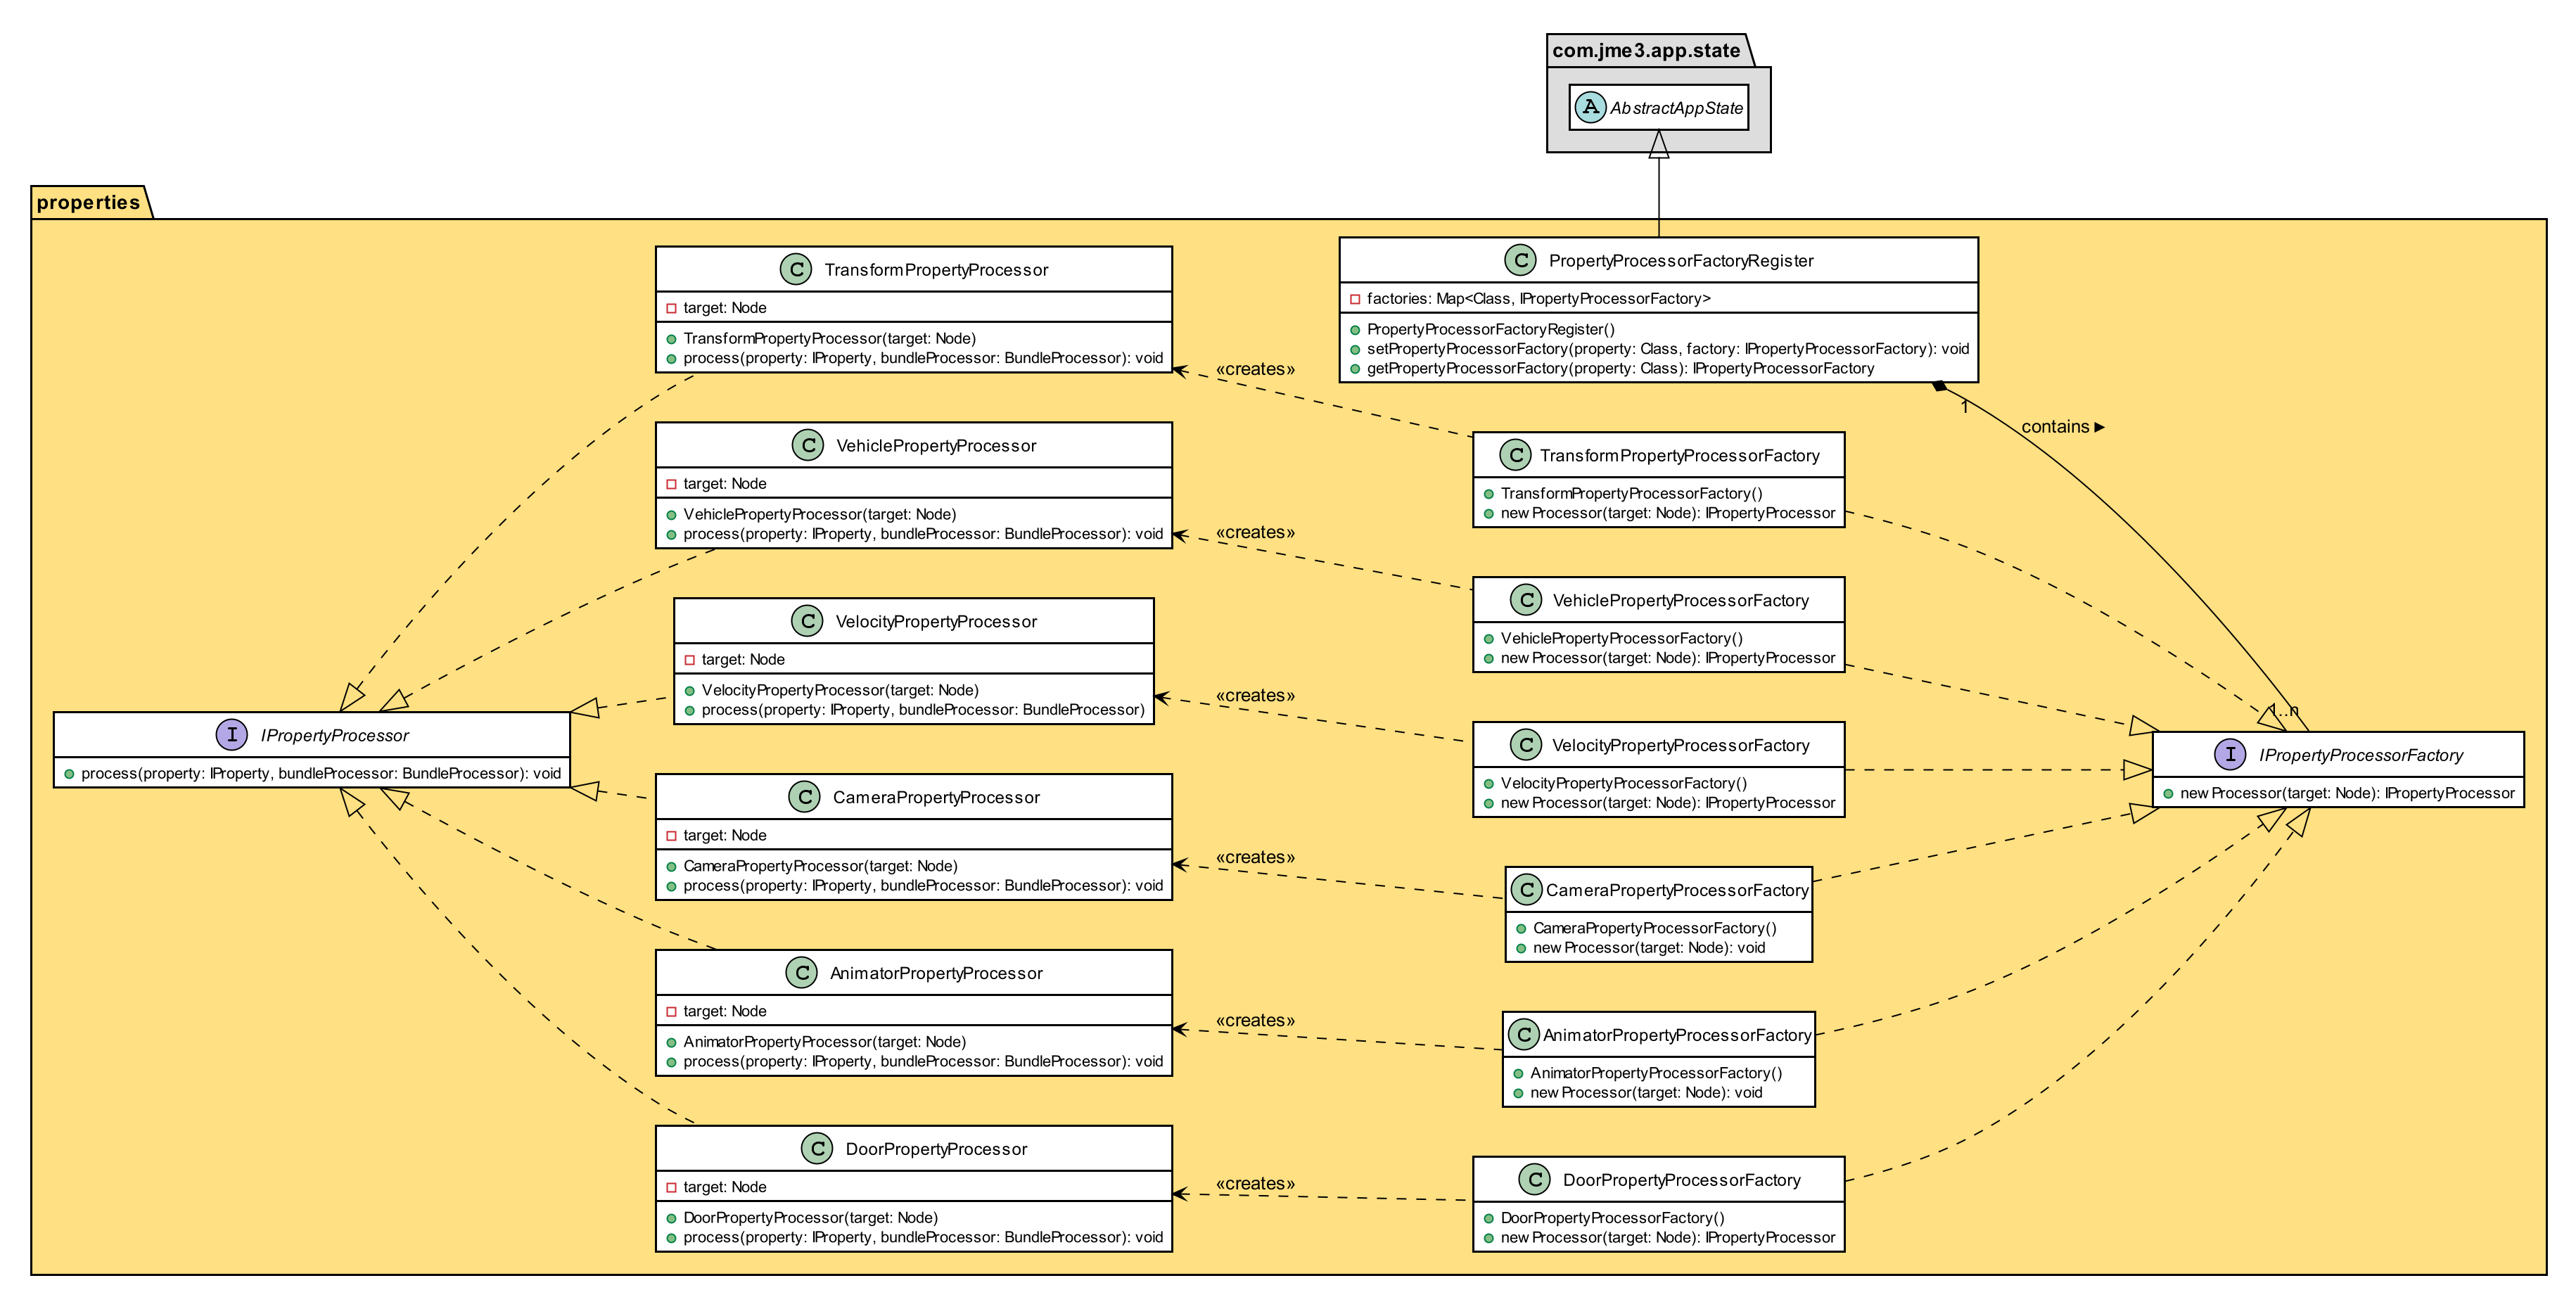
\includegraphics[width=0.9\linewidth]{Interface/render-tick-dynamics-properties.png}
        \caption{rendering.tick.dynamics.properties Klassen-Diagram}
    \end{figure}

    \paragraph{\underline{IPropertyProcessor}} \mbox{}\\
    \\
    Interface welches die Funktionalität für die Verarbeitung von \textit{IProperty}s.\par

        \textbf{Methoden}
        \begin{itemize}
            \item  \textit{+ process(IProperty property, DynamicGameObjectProcessor dgoProcessor): void}
                \begin{leftbar}[0.9\linewidth]
                    Verarbeitet die gegebene \textit{IProperty}.\\
                    \textbf{@param property} die \textit{IProperty} welche verarbeitet werden soll.\\
                    \textbf{@param dgoProcessor} der \textit{DynamicGameObjectProcessor} welcher die Methode aufgerufen hat.\\
                    \textbf{@throws IllegalStateException} falls die gegebene \textit{IProperty} nicht von diesem \textit{IPropertyProcessor}
                    bearbeitet werden kann.
                \end{leftbar}
        \end{itemize}

    \pagebreak
    \paragraph{\underline{IPropertyProcessorFactory}} \mbox{}\\
    \\
    Interface für Fabriken von \textit{IPropertyProcessor}s.\par

        \textbf{Methoden}
        \begin{itemize}
            \item \textit{+ newProcessor(Node target): IPropertyProcessor}
                \begin{leftbar}[0.9\linewidth]
                    Erstellt einen neuen \textit{IPropertyProcessor} welcher auf der gegebenen \textit{Node} arbeitet.\\
                    \textbf{@param target} die \textit{Node}, auf welcher der \textit{IPropertyProcessor} arbeiten soll.
                    \textbf{@return} der neu erstellte \textit{IPropertyProcessor}.
                \end{leftbar}
        \end{itemize}

    \paragraph{\underline{TransformPropertyProcessor}} \mbox{}\\
    \\
    \textit{IPropertyProcessor} für \textit{TransformProperty}s.\par

        \textbf{Attribute}
        \begin{itemize}
            \item \textit{+ Node target}
                \begin{leftbar}[0.9\linewidth]
                    Die \textit{Node} auf welcher dieser \textit{TransformPropertyProcessor} arbeitet.
                \end{leftbar}
        \end{itemize}
        \textbf{Methoden}
        \begin{itemize}
            \item \textit{+ TransformPropertyProcessor(Node target)}
                \begin{leftbar}[0.9\linewidth]
                    Erstellt einen neuen \textit{TransformPropertyProcessor}.\\
                    \textbf{@param target} die \textit{Node} auf welcher dieser \textit{TransformPropertyProcessor} arbeitet.
                \end{leftbar}
            \item \textit{+ process(IProperty property, DynamicGameObjectProcessor dgoProcessor): void}
                \begin{leftbar}[0.9\linewidth]
                    Siehe \textit{IPropertyProcessor.process()}.
                \end{leftbar}
        \end{itemize}

    \paragraph{\underline{TransformPropertyProcessorFactory}} \mbox{}\\
    \\
    Fabrik für \textit{TransformPropertyProcessor}s.\par

        \textbf{Methoden}
        \begin{itemize}
            \item \textit{+ TransformPropertyProcessorFactory()}
                \begin{leftbar}[0.9\linewidth]
                    Erstellt eine neue \textit{TransformPropertyProcessorFactory}.
                \end{leftbar}
            \item \textit{+ newProcessor(Node target): IPropertyProcessor}
                \begin{leftbar}[0.9\linewidth]
                    Siehe \textit{IPropertyProcessorFactory.newProcessor()}.
                \end{leftbar}
        \end{itemize}

    \paragraph{\underline{VelocityPropertyProcessor}} \mbox{}\\
    \\
    \textit{IPropertyProcessor} für \textit{VelocityProperty}s.\par

        \textbf{Attribute}
        \begin{itemize}
            \item \textit{+ Node target}
                \begin{leftbar}[0.9\linewidth]
                    Die \textit{Node} auf welcher dieser \textit{VelocityPropertyProcessor} arbeitet.
                \end{leftbar}
        \end{itemize}
        \textbf{Methoden}
        \begin{itemize}
            \item \textit{+ VelocityPropertyProcessor(Node target)}
                \begin{leftbar}[0.9\linewidth]
                    Erstellt einen neuen \textit{VelocityPropertyProcessor}.\\
                    \textbf{@param target} die \textit{Node} auf welcher dieser \textit{VelocityPropertyProcessor} arbeitet.
                \end{leftbar}
            \item \textit{+ process(IProperty property, DynamicGameObjectProcessor dgoProcessor): void}
                \begin{leftbar}[0.9\linewidth]
                    Siehe \textit{IPropertyProcessor.process()}.
                \end{leftbar}
        \end{itemize}

    \paragraph{\underline{VelocityPropertyProcessorFactory}} \mbox{}\\
    \\
    Fabrik für \textit{VelocityPropertyProcessor}s.\par

        \textbf{Methoden}
        \begin{itemize}
            \item \textit{+ VelocityPropertyProcessorFactory()}
                \begin{leftbar}[0.9\linewidth]
                    Erstellt eine neue \textit{VelocityPropertyProcessorFactory}.
                \end{leftbar}
            \item \textit{+ newProcessor(Node target): IPropertyProcessor}
                \begin{leftbar}[0.9\linewidth]
                    Siehe \textit{IPropertyProcessorFactory.newProcessor()}.
                \end{leftbar}
        \end{itemize}

    \paragraph{\underline{CameraPropertyProcessor}} \mbox{}\\
    \\
    \textit{IPropertyProcessor} für \textit{CameraProperty}s.\par

        \textbf{Attribute}
        \begin{itemize}
            \item \textit{+ Node target}
                \begin{leftbar}[0.9\linewidth]
                    Die \textit{Node} auf welcher dieser \textit{CameraPropertyProcessor} arbeitet.
                \end{leftbar}
        \end{itemize}

        \pagebreak
        \textbf{Methoden}
        \begin{itemize}
            \item \textit{+ CameraPropertyProcessor(Node target)}
                \begin{leftbar}[0.9\linewidth]
                    Erstellt einen neuen \textit{CameraPropertyProcessor}.\\
                    \textbf{@param target} die \textit{Node} auf welcher dieser \textit{CameraPropertyProcessor} arbeitet.
                \end{leftbar}
            \item \textit{+ process(IProperty property, DynamicGameObjectProcessor dgoProcessor): void}
                \begin{leftbar}[0.9\linewidth]
                    Siehe \textit{IPropertyProcessor.process()}.
                \end{leftbar}
        \end{itemize}

    \paragraph{\underline{CameraPropertyProcessorFactory}} \mbox{}\\
    \\
    Fabrik für \textit{CameraPropertyProcessor}s.\par

        \textbf{Methoden}
        \begin{itemize}
            \item \textit{+ CameraPropertyProcessorFactory()}
                \begin{leftbar}[0.9\linewidth]
                    Erstellt eine neue \textit{CameraPropertyProcessorFactory}.
                \end{leftbar}
            \item \textit{+ newProcessor(Node target): IPropertyProcessor}
                \begin{leftbar}[0.9\linewidth]
                    Siehe \textit{IPropertyProcessorFactory.newProcessor()}.
                \end{leftbar}
        \end{itemize}

    \paragraph{\underline{VehiclePropertyProcessor}} \mbox{}\\
    \\
    \textit{IPropertyProcessor} für \textit{VehicleProperty}s.\par

        \textbf{Attribute}
        \begin{itemize}
            \item \textit{+ Node target}
                \begin{leftbar}[0.9\linewidth]
                    Die \textit{Node} auf welcher dieser \textit{VehiclePropertyProcessor} arbeitet.
                \end{leftbar}
        \end{itemize}
        \textbf{Methoden}
        \begin{itemize}
            \item \textit{+ VehiclePropertyProcessor(Node target)}
                \begin{leftbar}[0.9\linewidth]
                    Erstellt einen neuen \textit{VehiclePropertyProcessor}.\\
                    \textbf{@param target} die \textit{Node} auf welcher dieser \textit{VehiclePropertyProcessor} arbeitet.
                \end{leftbar}
            \item \textit{+ process(IProperty property, DynamicGameObjectProcessor dgoProcessor): void}
                \begin{leftbar}[0.9\linewidth]
                    Siehe \textit{IPropertyProcessor.process()}.
                \end{leftbar}
        \end{itemize}

    \pagebreak
    \paragraph{\underline{VehiclePropertyProcessorFactory}} \mbox{}\\
    \\
    Fabrik für \textit{VehiclePropertyProcessor}s.\par

        \textbf{Methoden}
        \begin{itemize}
            \item \textit{+ VehiclePropertyProcessorFactory()}
                \begin{leftbar}[0.9\linewidth]
                    Erstellt eine neue \textit{VehiclePropertyProcessorFactory}.
                \end{leftbar}
            \item \textit{+ newProcessor(Node target): IPropertyProcessor}
                \begin{leftbar}[0.9\linewidth]
                    Siehe \textit{IPropertyProcessorFactory.newProcessor()}.
                \end{leftbar}
        \end{itemize}

    \paragraph{\underline{AnimatorPropertyProcessor}} \mbox{}\\
    \\
    \textit{IPropertyProcessor} für \textit{AnimatorProperty}s.\par

        \textbf{Attribute}
        \begin{itemize}
            \item \textit{+ Node target}
                \begin{leftbar}[0.9\linewidth]
                    Die \textit{Node} auf welcher dieser \textit{AnimatorPropertyProcessor} arbeitet.
                \end{leftbar}
        \end{itemize}
        \textbf{Methoden}
        \begin{itemize}
            \item \textit{+ AnimatorPropertyProcessor(Node target)}
                \begin{leftbar}[0.9\linewidth]
                    Erstellt einen neuen \textit{AnimatorPropertyProcessor}.\\
                    \textbf{@param target} die \textit{Node} auf welcher dieser \textit{AnimatorPropertyProcessor} arbeitet.
                \end{leftbar}
            \item \textit{+ process(IProperty property, DynamicGameObjectProcessor dgoProcessor): void}
                \begin{leftbar}[0.9\linewidth]
                    Siehe \textit{IPropertyProcessor.process()}.
                \end{leftbar}
        \end{itemize}

    \paragraph{\underline{AnimatorPropertyProcessorFactory}} \mbox{}\\
    \\
    Fabrik für \textit{AnimatorPropertyProcessor}s.\par

        \textbf{Methoden}
        \begin{itemize}
            \item \textit{+ AnimatorPropertyProcessorFactory()}
                \begin{leftbar}[0.9\linewidth]
                    Erstellt eine neue \textit{AnimatorPropertyProcessorFactory}.
                \end{leftbar}
            \item \textit{+ newProcessor(Node target): IPropertyProcessor}
                \begin{leftbar}[0.9\linewidth]
                    Siehe \textit{IPropertyProcessorFactory.newProcessor()}.
                \end{leftbar}
        \end{itemize}

    \pagebreak
    \paragraph{\underline{DoorPropertyProcessor}} \mbox{}\\
    \\
    \textit{IPropertyProcessor} für \textit{DoorProperty}s.\par

        \textbf{Attribute}
        \begin{itemize}
            \item \textit{+ Node target}
                \begin{leftbar}[0.9\linewidth]
                    Die \textit{Node} auf welcher dieser \textit{DoorPropertyProcessor} arbeitet.
                \end{leftbar}
        \end{itemize}
        \textbf{Methoden}
        \begin{itemize}
            \item \textit{+ DoorPropertyProcessor(Node target)}
                \begin{leftbar}[0.9\linewidth]
                    Erstellt einen neuen \textit{DoorPropertyProcessor}.\\
                    \textbf{@param target} die \textit{Node} auf welcher dieser \textit{DoorPropertyProcessor} arbeitet.
                \end{leftbar}
            \item \textit{+ process(IProperty property, DynamicGameObjectProcessor dgoProcessor): void}
                \begin{leftbar}[0.9\linewidth]
                    Siehe \textit{IPropertyProcessor.process()}.
                \end{leftbar}
        \end{itemize}

    \paragraph{\underline{DoorPropertyProcessorFactory}} \mbox{}\\
    \\
    Fabrik für \textit{DoorPropertyProcessor}s.\par

        \textbf{Methoden}
        \begin{itemize}
            \item \textit{+ DoorPropertyProcessorFactory()}
                \begin{leftbar}[0.9\linewidth]
                    Erstellt eine neue \textit{DoorPropertyProcessorFactory}.
                \end{leftbar}
            \item \textit{+ newProcessor(Node target): IPropertyProcessor}
                \begin{leftbar}[0.9\linewidth]
                    Siehe \textit{IPropertyProcessorFactory.newProcessor()}.
                \end{leftbar}
        \end{itemize}

    \pagebreak
    \paragraph{\underline{PropertyProcessorFactoryRegister}} \mbox{}\\
    \\
    \textit{Appstate}, welcher alls bekannten \textit{IPropertyProcessorFactory}s hält.\par

        \textbf{Methoden}
        \begin{itemize}
            \item \textit{+ PropertyProcessorFactoryRegister()}
                \begin{leftbar}[0.9\linewidth]
                    Erstellt ein neues \textit{PropertyProcessorFactoryRegister} und initialisiert factories als leere Map.
                \end{leftbar}
            \item \textit{+ setPropertyProcessorFactory(Class<? extends IProperty> property, IPropertyProcessorFactory factory): void}
                \begin{leftbar}[0.9\linewidth]
                    Setzt die \textit{IPropertyProcessorFactory}, welche verwendet wird um \textit{IPropertyProcessor}s für eine \textit{IProperty} vom gegebenen Typ
                    zu erstellen.\\
                    \textbf{@param property} der Typ von \textit{IProperty} für den diese \textit{IPropertyProcessorFactory} verwendet werden soll.\\
                    \textbf{@param factory} die \textit{IPropertyProcessorFactory}.
                \end{leftbar}
            \item \textit{+ getPropertyProcessorFactory(Class<? extends IProperty> property): IPropertyProcessorFactory}
                \begin{leftbar}[0.9\linewidth]
                    Liefert die \textit{IPropertyProcessorFactory}, welche für den gegebenen Typ von \textit{IProperty} verwendet werden soll.\\
                    \textbf{@param property} der Typ von \textit{IProperty} für den die \textit{IPropertyProcessorFactory} gesucht ist.\\
                    \textbf{@return} die \textit{IPropertyProcessorFactory} für den gegebenen Typ von \textit{IProperty} oder null falls keine
                    \textit{IPropertyProcessorFactory} für diesen Typ gesetzt wurde.
                \end{leftbar}
        \end{itemize}